\section{Networking with LuaSocket}

Author: Matthew Frazier
\href{mailto:leafstormrush@gmail.com}{\texttt{leafstormrush@gmail.com}}

The most common library for networking in Lua is
\href{http://w3.impa.br/~diego/software/luasocket/}{LuaSocket} by
Diego Nehab. In addition to low-level support for communicating
directly through sockets, it also includes:

\begin{itemize}
\item
  HTTP client
\item
  FTP client
\item
  SMTP client
\item
  Mail processing filters
\item
  URL manipulating functions
\end{itemize}
LuaSocket is installable via LuaRocks, as explained in
:ref:`luarocks`. Many distributions also provide LuaSocket
packages.

\begin{TODO}Fix references\end{TODO}

\subsection{Socket-Level Programming}

To create a TCP socket%
\footnote{There's also UDP, but we're not covering it in this introduction.}
connected to a particular place, you can use \verb!socket.connect!,
like this:

\begin{LUA}
require 'socket'
local sock = socket.connect("www.example.com", 80)
\end{LUA}

From there, you can send and receive on the socket object.

\begin{LUA}
sock:send("GET / HTTP/1.0\n\n")
local data = sock:recv()
\end{LUA}

You could also use \verb!socket.tcp("www.example.com", 80)! and
then \verb!connect! it separately, but this is a shortcut.

\subsection{Servers}

Servers are \emph{cool!} According to some guy we met:

\begin{QUOTE}
Servers are the whole reason the Internet exists as we know it.
\end{QUOTE}

You can create servers by using \verb!socket.bind!.

Here is a graph about servers.

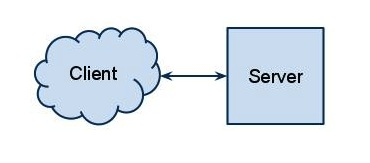
\includegraphics{20-networking/01-server-graph.jpg}

\subsubsection{Concurrency}

Everyone is talking about concurrency these days!

Some of the ways people have thought of for being concurrent are:

\begin{enumerate}
\item
  Multithreading.
\item
  Having multiple processes.
\item
  Asynchronous programming.
\end{enumerate}

Fortunately, Lua has something cool you can use for number three:
Coroutines! (If you don't know about coroutines, see
:ref:`using-coroutines` for more info.)

\subsection{Glossary}

\begin{description}

\item[client]
The program run by the user that talks to clients.

\item[server]
The program that clients talk to.

\item[TCP]
What most people use nowadays instead of UDP.

\end{description}
